\documentclass[11pt]{article}
\usepackage[T1]{fontenc}
\usepackage[utf8]{inputenc} 
\usepackage[polish]{babel}    
\usepackage{hyperref}
\usepackage{indentfirst}
\usepackage[backend=biber, sorting=none]{biblatex}
\addbibresource{main.bib}
\usepackage{csquotes}
\usepackage{graphicx}
\usepackage{amsmath}
\usepackage{blindtext}
\usepackage{tocbibind}


\newcounter{boxlblcounter}  
\newcommand{\makeboxlabel}[1]{\fbox{#1.}\hfill}% \hfill fills the label box
\newenvironment{boxlabel}
  {\begin{list}
    {\arabic{boxlblcounter}}
    {\usecounter{boxlblcounter}
     \setlength{\labelwidth}{3em}
     \setlength{\labelsep}{0em}
     \setlength{\itemsep}{2pt}
     \setlength{\leftmargin}{1.5cm}
     \setlength{\rightmargin}{2cm}
     \setlength{\itemindent}{0em} 
     \let\makelabel=\makeboxlabel
    }
  }
{\end{list}}


\title{Projekt 1 - wskaźnik MACD}
\date{marzec 2025}
\author{Mikołaj Wiszniewski \\ s197925, gr.5}

\begin{document}
    \maketitle

    \renewcommand*\contentsname{Spis treści}
    \tableofcontents{}

    \newpage


    \section{Wstęp do projektu}

    \subsection{Cel}
    Celem projektu jest analiza skuteczności strategii inwestycyjnej opartej na wskaźniku MACD (\hyperlink{def:macd}{definicja w sekcji \textbf{2.1}}). Badanie obejmie identyfikację zalet i ograniczeń tego narzędzia oraz ocenę jego wpływu na potencjalne zyski inwestora stosującego tę metodę
    
    \subsection{Założenia}
    Ze względu na szczegółowość analizy wskaźnika, ważne są założenia co do implementacji algorytmu symulującego jego wydajność. 
    Przeprowadzane operacje będą dotyczyły wartości całego portfolio, tzn. kupujemy za całą gotówkę jaką posiadamy, a przy sprzedaży likwidujemy wszystkie posiadane aktywa.
    Profit zyskany na transakcji jest obliczany tylko i wyłącznie w oparciu o cenę zamknięcia analizowanego okresu, nie bierze pod uwagę ewentualnego poślizgu cenowego (\textit{ang. slippage}) ani ewentualnych opłat pośrednika.


    \section{Wprowadzenie teoretyczne}

    \subsection{Czym jest MACD?}

    \hypertarget{def:macd}{MACD}(\textit{Moving Average Convergence/Divergence})\cite{wiki:MACD} - wskaźnik do analizy technicznej skonstruowany w roku 1979.
    Identyfikuje trendy rozpoczynające się na rynku poprzez badanie zbieżności i rozbieżności średnich kroczących, co przedstawiają wzory \eqref{eq:wzory} oraz \eqref{eq:wzory2}.Proste średnie kroczące, zwane również średnimi ruchomymi\cite{wiki:Średnia_ruchoma} to zwykłe średnie arytmetyczne wartości ostatnich $n$ okresów.
    
    Jest niezwykle popularny zarówno wśród graczy giełdowych, jak i inwestorów, do badania sygnałów kupna i sprzedaży aktywów.

    Wartość MACD jest obliczana na podstawie następujących wzorów:
    \begin{gather}
        EMA_N = \frac{p_0 + (1 - \alpha)p_1 + (1-\alpha)^2p_2 + \cdots + (1-\alpha)^Np_N}{1 + (1 - \alpha) + (1-\alpha)^2 + \cdots + (1-\alpha)^N}\\
        \label{eq:wzory}
        \text{MACD} = \text{EMA}_{12} - \text{EMA}_{26}\\
        \label{eq:wzory2}
        \text{SIGNAL} = \text{EMA}_{9}(\text{MACD})
    \end{gather}
    gdzie:
    \begin{itemize}
        \item $p_i$ to cena instrumentu z dnia \textit{i}
        \item $\alpha = \frac{2}{N+1}$
        \item $N$ - liczba analizowanych ram czasowych
        \item EMA$_k$ - średnia krocząca z ostatnich $k$ ram
        \item SIGNAL - 9-ramowa średnia krocząca z MACD
    \end{itemize}

    \subsection{Opis strategii}
    Analizowane są dwie średnie kroczące - MACD oraz SIGNAL. 
    Ich każdorazowe przecięcie oznacza sygnał do kupna lub sprzedaży.
    Ustalenie co do kierunku naszej transakcji przebiega w następujący sposób. Jeżeli linia MACD przecina SIGNAL od góry jest to sygnał do zakupu (oraz pośrednio zapowiedź trendu wzrostu), a w przeciwnym przypadku dokonujemy sprzedaży.


    \section{Analiza zachowania wskaźnika}

    \subsection{Bitcoin względem USD}
    \begin{center}\hypertarget{png:btcusd}{}
        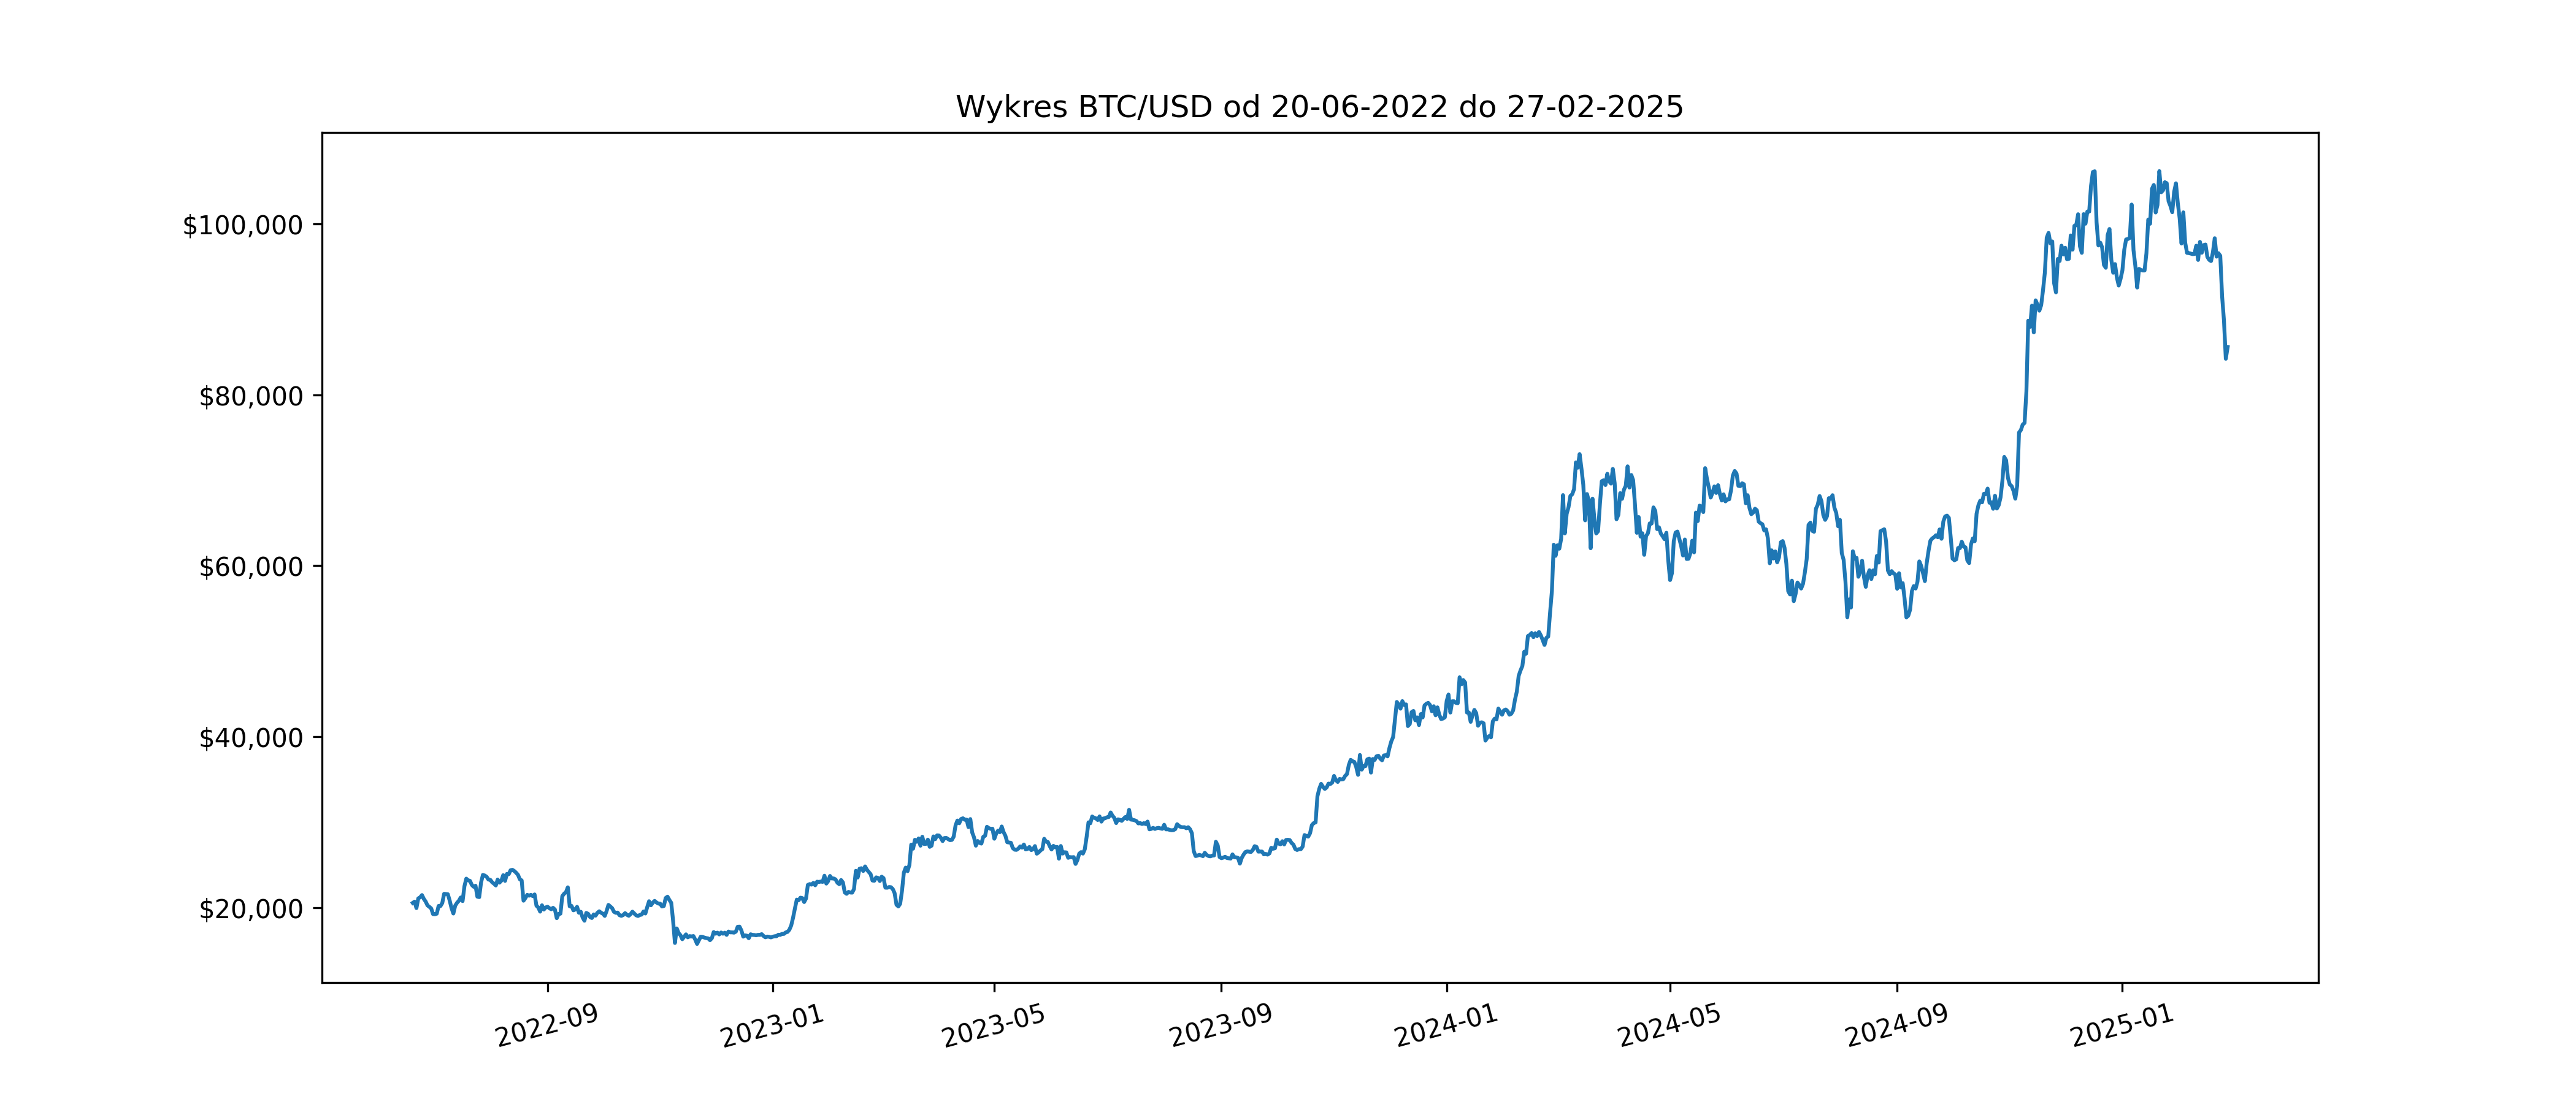
\includegraphics[width=1\textwidth]{btc_plot.png}
    \end{center}
    
    Powyższy wykres przedstawia ceny zamknięcia poszczególnych dni Bitcoin'a względem dolara amerykańskieg (dane\cite{data:btc}).
    W latach 2022 i 2023 inwestorzy nie wykazywali zainteresowania instrumentem, obrót był niski, a co za tym idzie zmienność ceny (\textit{ang. volatility}) również. 
    W roku 2024, gdy BTC zaczął wykazywać silny trend wzrostowy, publika zmieniła opinię, a wolumen wraz ze zmiennością zdecydowanie się zwiększyły. 
    
    \begin{center}
        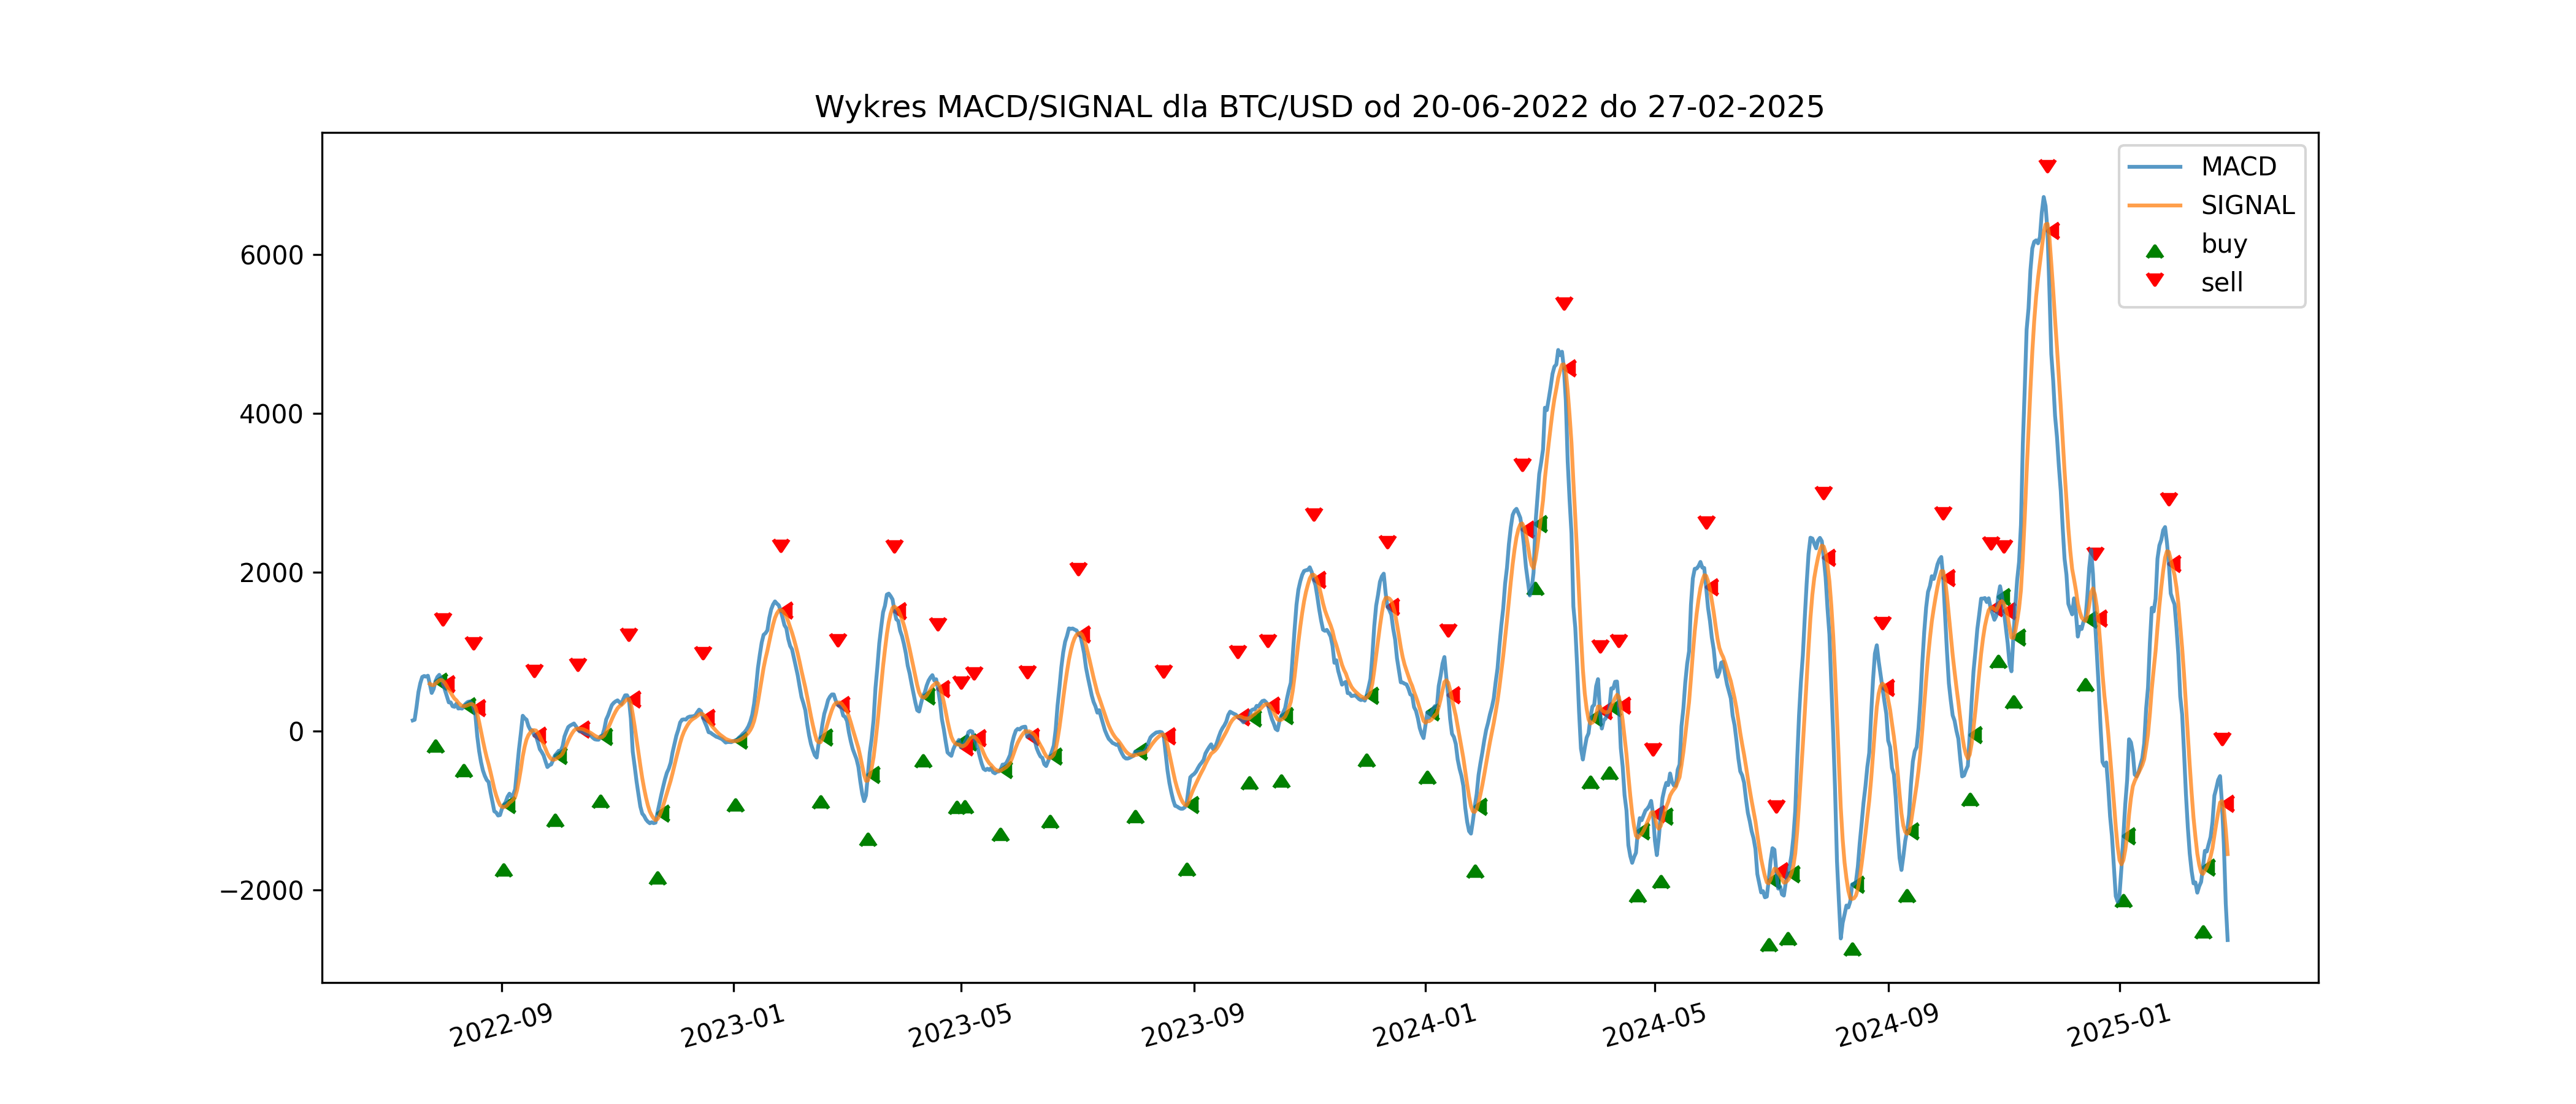
\includegraphics[width=1\textwidth]{signals_plot.png}
    \end{center}

    Zielone trójkąty odpowiadają sygnałom kupna, a czerwone sprzedaży.
    Sama informacja o tym jak wyglądają średnie na przestrzeni analizowanego czasu nie daje informacji o wydajności strategii. Można zauważyć, że wspomniana wcześniej zmienność ceny ma swoje odwzorowanie w zmienności wartości wskaźnika, a co za tym idzie - jego wydajności.


    \subsubsection{Interpretacja szczegółowa}
    \begin{center}
        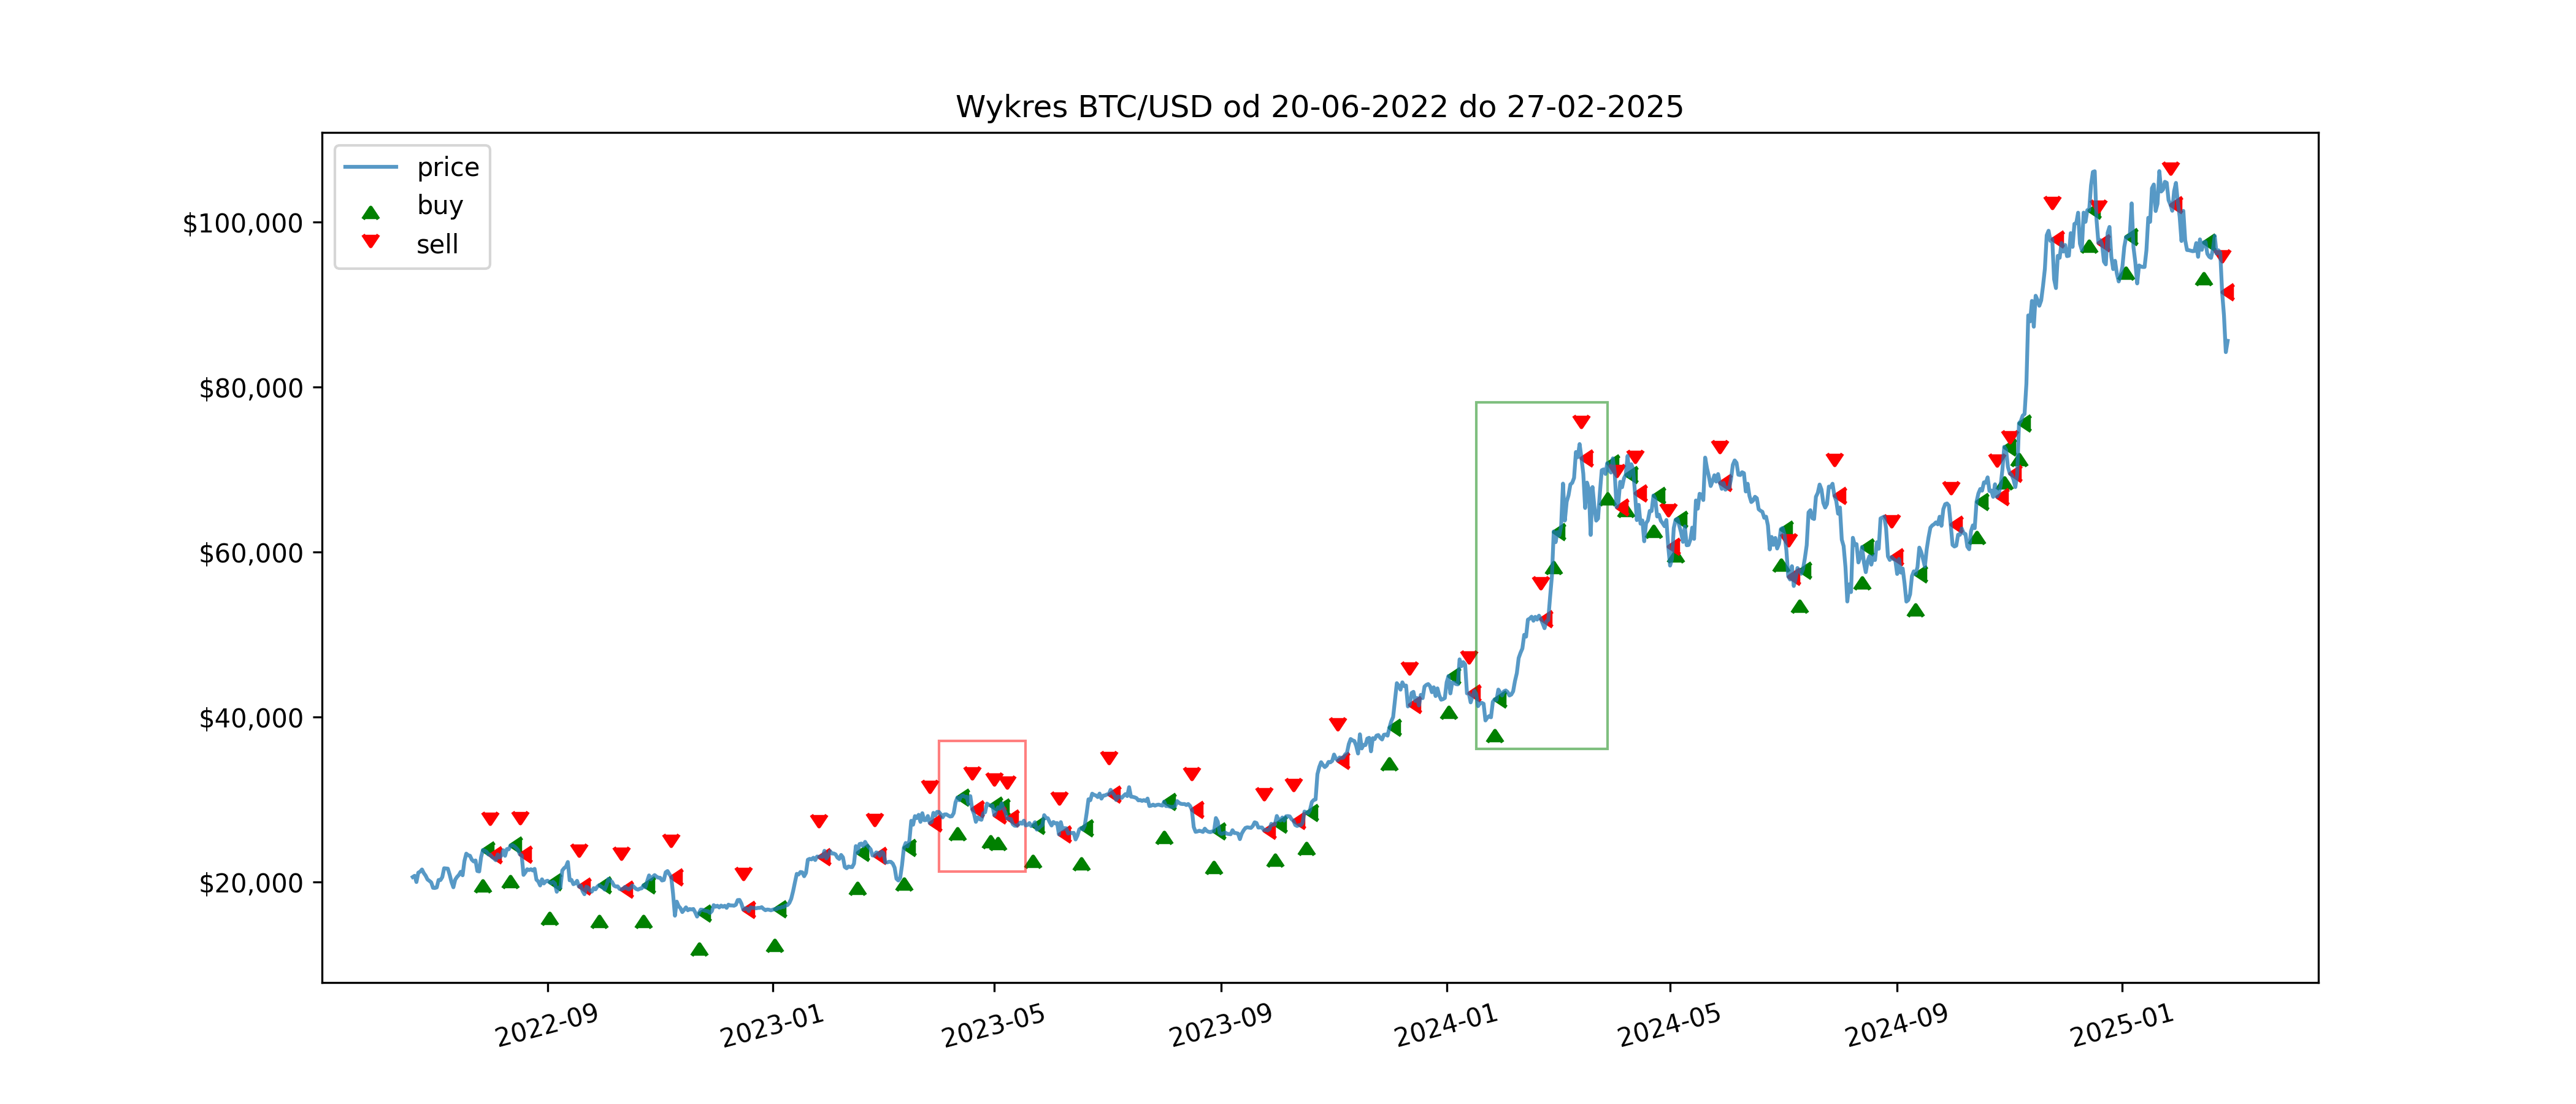
\includegraphics[width=1\textwidth]{btc_plot_with_signals.png}
    \end{center}

    Na \hyperlink{png:btcusd}{wykres BTC/USD} nałożone zostały sygnały dostarczone przez wskaźnik. 
    Widniejące na nim prostokąty pokazują przykładowe transakcje, zielony - zyskowne oraz czerwony - stratne, które będą dogłębniej przeanalizowane w tej sekcji.
    
    Można zauważyć, że MACD sygnalizuje bardzo dużo transakcji. 
    Gdy zmienność jest niska, kupno oraz sprzedaż dokonują się na przeważnie podobnym poziomie, natomiast w przypadku trendu wzrostowego i zwiększonej zmienności sygnały wyglądają dużo lepiej. Kupna są dokonywane w lokalnych dołkach, natomiast sprzedaże po zapowiedzi spadku z wierzchołka.
    
    \begin{center}
        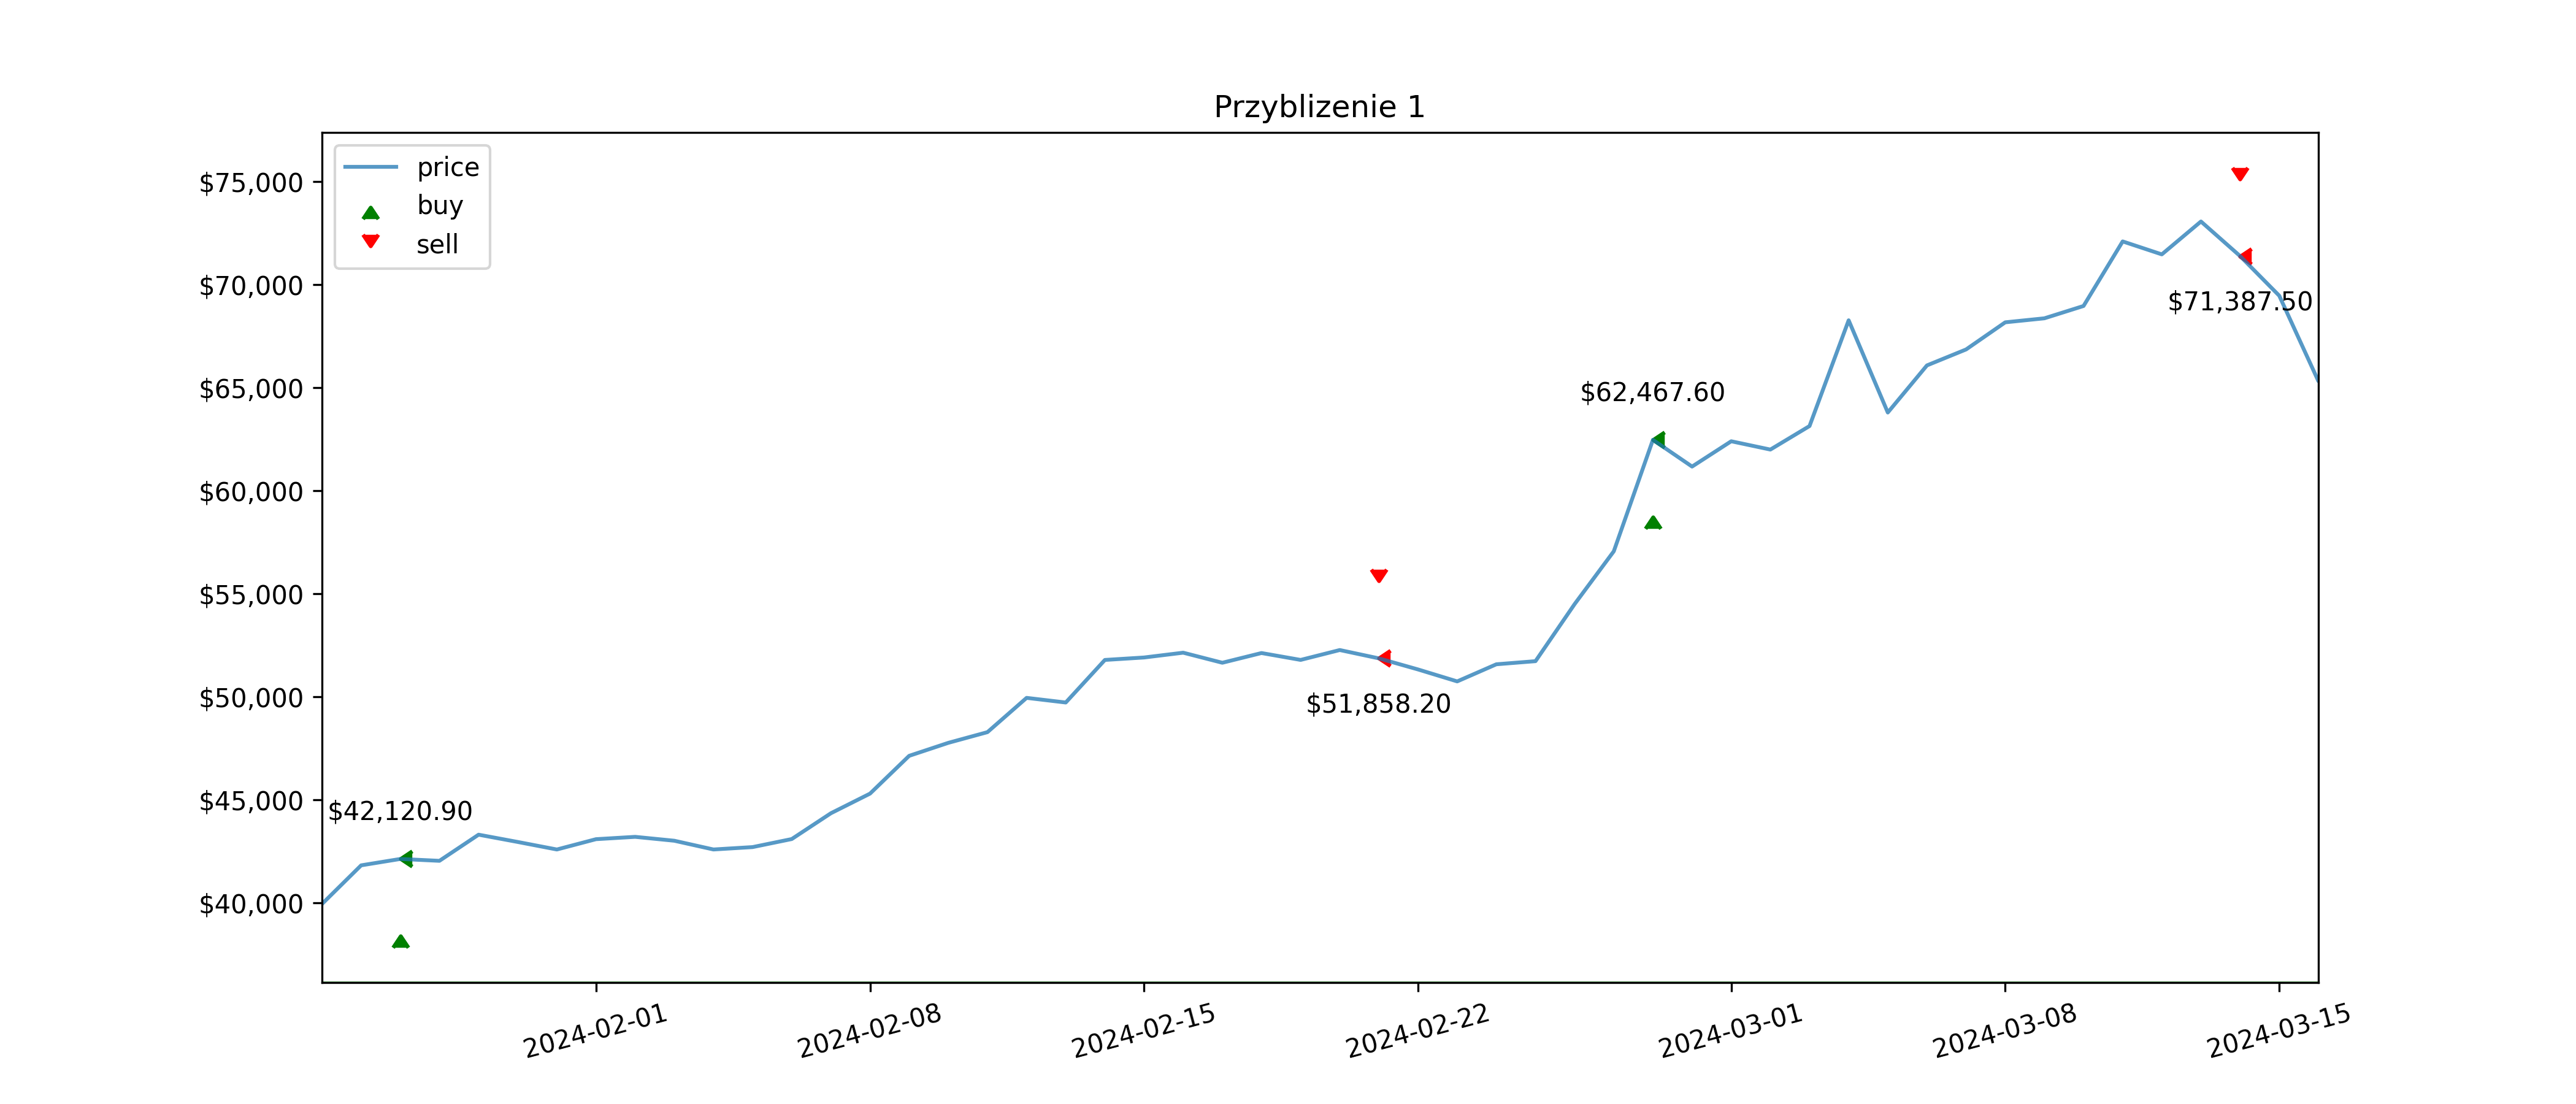
\includegraphics[width=1\textwidth]{zoomed1.png}
    \end{center}

    Pierwsze przybliżenie ukazuje zakres dat, w którym cena wykazuje wyraźny trend zwyżkowy. 
    Wskaźnik zasygnalizował wykonanie dwóch transakcji:
    \begin{boxlabel}
        \item Cena otwarcia $\$51,858.20$, cena zamknięcia $\$42,120.90$, profit $+23\%$.
        \item Cena otwarcia $\$62,467.60$, cena zamknięcia $\$71,387.50$, profit $+14\%$. 
    \end{boxlabel}
    
    Zysk łączny $+40\%$.
    Na myśl nasuwa się wniosek, że wskaźnik świetnie sobie radzi podczas jednoznacznego trendu.
    Należy jednak mieć na uwadze, że podczas analizowanego okresu cena instrumentu wzrosła aż o $80\%$. 
    Pokazuje to, że pomimo ruchu zwyżkowego ceny, wskaźnik nie był w stanie "złapać" go całego, a jedynie część.
    Dla bardzo konswerwatywnego inwestora może to być jednak zaleta MACD, ze względu na częstą realizację zysków, co znacznie minimalizuje ryzyko.
    \begin{center}
        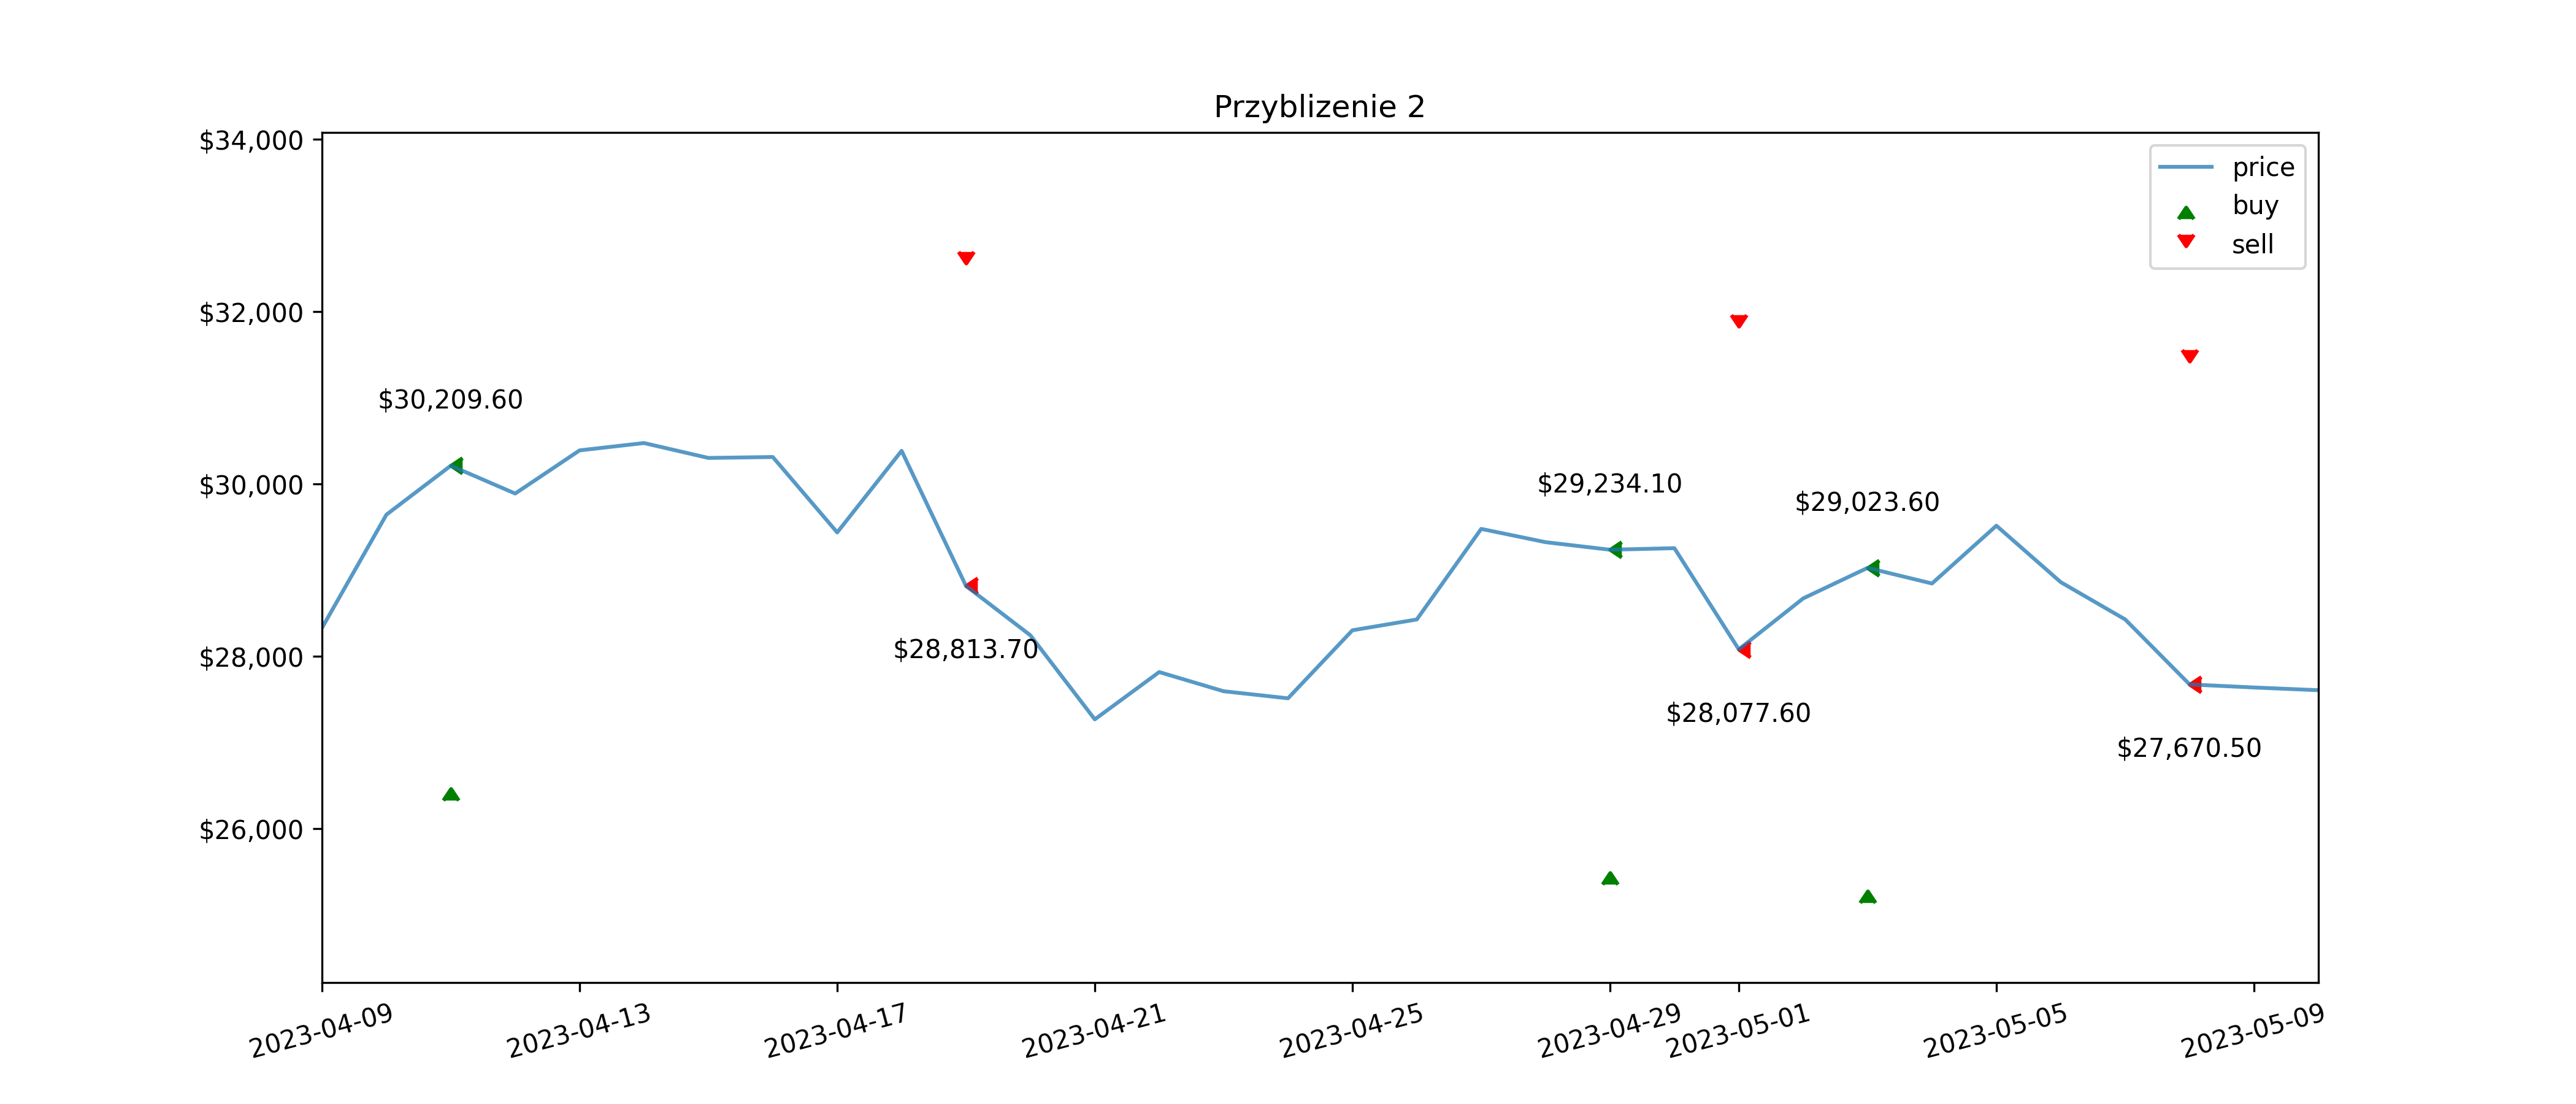
\includegraphics[width=1\textwidth]{zoomed2.png}
    \end{center}
    
    Powyższy wykres pokazuje 6 transakcji, czyli 3 zamknięcia pozycji, z których wszystkie były na stracie.
    Pokazuje to słabość strategii w momencie, gdy cena wykazuje trend boczny.
    
    Przy każdym wzroście, wskaźnik informuje o nadchodzącym ruchu w górę, natomiast przy gwałtowniejszym spadku uważa, że rozpoczyna się trend spadkowy i sprzedaje aktywa na stracie.
    Może to doprowadzić do szkód, gdy stagnacja cenowa się przedłuży i wskaźnik będzie sygnalizował wiele transakcji kończących się na niewielkiej, a sumarycznie dużej, utracie kapitału.

    \begin{boxlabel}
        \item Cena otwarcia $\$30,209.60$, cena zamknięcia $\$28,813.70$, profit $-4.7\%$.
        \item Cena otwarcia $\$29,234.10$, cena zamknięcia $\$28,077.60$, profit $-4\%$.
        \item Cena otwarcia $\$29,023.60$, cena zamknięcia $\$27,670.50$, profit $-4.7\%$
    \end{boxlabel}
    
    Łączna strata $-12.8\%$. Strategia spowodowała dość znaczące straty w portfelu, gdy ruchy cenowe nie wykazywały trendu spadkowego.
    Jest to definitywnie wada MACD.

    \section{Symulacja}
    \subsection{porównanie ze strategią hold}
    
    \begin{center}
        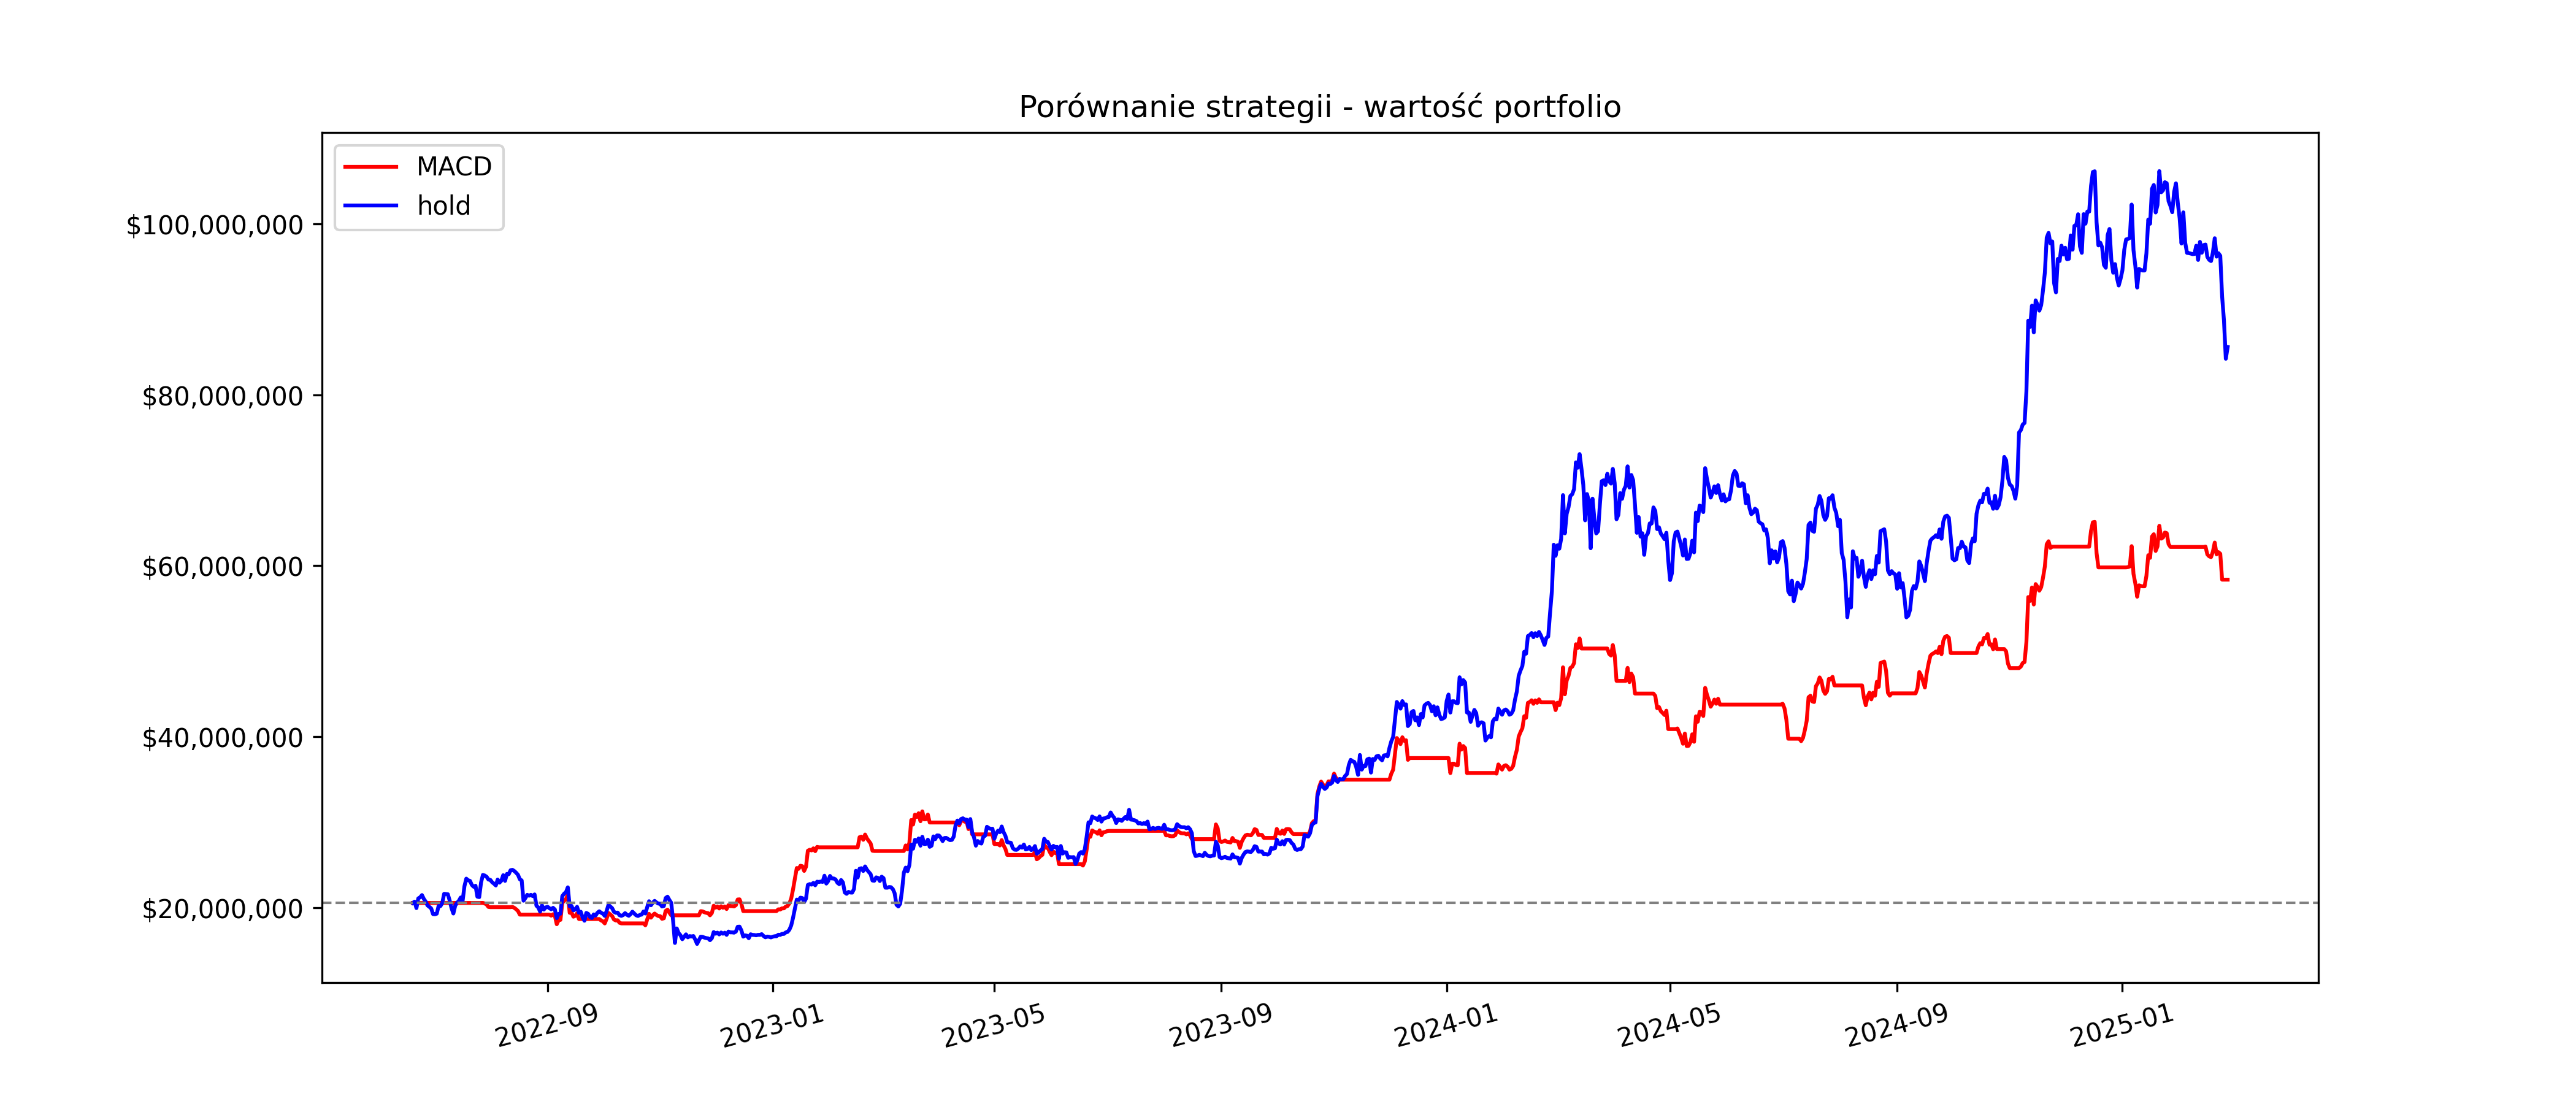
\includegraphics[width=1\textwidth]{compare_strategies.png}
    \end{center}
    \subsubsection{MACD}
    Stworzony algorytm na start do portfela otrzymuje ilość gotówki odpowiadającom 1000 Bitcoin'om, co w tym przypadku daje $\$20,572,300$.
    Maskymalna osiągnięta wartość portfiolio to $\$65,133,913$ (zysk $317\%$), a maksymalny spadek od wartości inicjalnej $-12.7\%$ (profit $-\$2,617,505$).
    Pod koniec działania posiada on $\$58,377,462$, co daje imponującą stopę zwrotu $284\%$.\\
    \\
    Algorytm wykonał łącznie 36 transakcji, z czego:
    
    17 było zyskownych, średni profit $\$4,178,210$.
    
    19 było stratnych, średni profit  $-\$1,748,653$.
    \\
    
    Współczynnik skuteczności transakcji wynosi $47.2\%$.
    Nie jest to zły wynik, szczególnie mając na uwadze to, że RR (\textit{ang. Risk/Reward Ratio}) wynosi $2.39$.
    W skrócie oznacza to, że średni zysk transakcji jest $2.39$ raza większy niż średnia strata, sugerując, że algorytm skutecznie zarządza kapitałem.
    \subsubsection{Kup i trzymaj}
    Innym bardziej tradycyjnym sposobem inwestowania jest strategia "Kup i trzymaj" (\textit{ang. buy and hold})\cite{wiki:hold}.
    W tym przypadku brana jest pod uwagę wartość 1000 Bitcoin'ów w analizowanym okresie.
    Gdy instrument osiągnął najwyższą cenę w historii, wartośc portfela wynosiła $\$106,157,200$ (zysk $516\%$).
    W przypadku lokalnego dołka strata wynosiła $-23.3\%$ (profit $-\$4,796,100$).
    Na koniec analizowanego okresu 1000 BTC jest warte $\$85,580,000$, a strategia daje zysk na poziomie $416\%$.

    \subsection{Wnioski}
    Wykres dobrze pokazuje wady oraz zalety MACD odwzorowane w wyżej przedstawionych danych.
    Strategia pośrednio posiada zabezpieczenie przed utratą kapitału, więc maksymalna strata jest zdecydowanie mniejsza w porównaniu ze strategią \textit{hold}, oznacza to jednak, że często będzie zbyt wcześnie zamykać pozycje, przegapiając duże ruchy cenowe. 
    
    MACD operuje na średnich kroczących, przez co dawane sygnały są opóźnione, a im większe tempo zmienności ceny, tym gorsze wyniki. 
    Widać to na wykresie, gdzie od początku roku 2024 (start rynku byka, zwiększenie dziennego obrotu) rozbieżność między wartościami portfeli drastycznie zaczęła się zwiększać.

    \section{Podsumowanie}
    Na podstawie przeprowadzonej symulacji oraz analizy w tym dokumencie nasuwa się wniosek, że strategia gry na giełdzie (lub rynku kryptowalut) oparta na wskaźniku MACD nie jest optymalna i nie może być nazwana kluczem do sukcesu na giełdzie.

    MACD jest wskaźnikiem przydatnym, jednak nikt nie powinien opierać całej swojej strategii wyłącznie na jego sygnałach.
    W praktyce często stosuje się go w połączeniu z innymi wskaźnikami, takimi jak RSI\cite{investopedia:rsi}.
    
    Główną wadą MACD jest jego opóźnienie względem rzeczywistych ruchów cenowych, co może prowadzić do niewykorzystania pełnego potencjału silnego trendu wzrostowego.
    Wynika to z jego zależności od średnich kroczących, która uniemożliwia całkowite wyeliminowanie opóźnienia w wysyłaniu sygnałów.
    
    Ponadto bardzo często generuje sygnały transakcyjne, co w rzeczywistości może skutkować zmniejszeniem zysków ze względu na koszty ich obsługi.
    Dodatkowo MACD może powodować zbyt szybkie zamykanie pozycji oraz straty kapitału w okresach trendu bocznego.

    Na strategię opartą na MACD mogą zdecydować się konserwatywni inwestorzy, którym zależy przede wszystkim na ochronie kapitału.
    Wiąże się to jednak z wieloma utrudnieniami i ograniczeniami.
    \newpage
    \printbibliography[
        heading=bibintoc,
        title={Bibliografia}
    ]
\end{document}

